\documentclass[12pt, a4paper]{article}
\usepackage[utf8]{inputenc}
\usepackage[english]{babel}
\usepackage{amsmath}
\usepackage{csquotes}
\usepackage{mathtools}
\usepackage{graphicx}
\usepackage{geometry}
\usepackage{setspace}
\usepackage{longtable}
\usepackage[style=authoryear]{biblatex}
\addbibresource{Bibliography.bib}

\geometry{top = 2.5cm, bottom = 2.5cm, left= 3cm, right= 3cm}

\title{Discharging of a Capacitor}
\author{Lee Farrugia \\ Experiment 0 \\ Group 1A}

\date{$15^{\text{th}}$ October 2021}

\begin{document}

\setstretch{1.5}

\maketitle

\section*{Aim:}
The aim of this experiment is to obtain two graphs and compare $V_0$ and $T$ between the linear fit and the exponential fit with the use of python.

\section*{Language and Packages:}
Python 3.9.7, Scipy.optimize, Numpy, Matplotlib.pyplot, Pandas

\section*{Data and Graphs:}

\begin{center}
\begin{longtable}{| c | c | c | c |}
    \caption{Voltage Discharge with Time Data} \label{tab:Table 1}\\    
    \hline \textbf{$t_1 {\text{/s}}$} & \textbf{$V_1 {\text{/V}}$} & \textbf{$t_2 {\text{/s}}$} & \textbf{$V_2 {\text{/V}}$} \\ \hline 
    
    \hline \textbf{\textpm\ 0.3} & \textbf{\textpm\ 0.01} & \textbf{\textpm\ 0.3} & \textbf{\textpm\ 0.01} \\ \hline 
    \endfirsthead
    
    \hline \textbf{$t_1 {\text{/s}}$} & \textbf{$V_1 {\text{/V}}$} & \textbf{$t_2 {\text{/s}}$} & \textbf{$V_2 {\text{/V}}$} \\ \hline

    \hline \textbf{\textpm\ 0.3} & \textbf{\textpm\ 0.01} & \textbf{\textpm\ 0.3} & \textbf{\textpm\ 0.01} \\ \hline
    \endhead
    
    \hline
    \endfoot
    
0.0 & 9.82 & 0.0 & 9.82 \\
20.0 & 8.03 & 20.0 & 8.04 \\
40.0 & 6.62 & 40.0 & 6.60 \\
60.0 & 5.44 & 60.0 & 5.46 \\
80.0 & 4.48 & 80.0 & 4.47 \\
100.0 & 3.70 & 100.0 & 3.71 \\
120.0 & 3.06 & 120.0 & 3.04 \\
140.0 & 2.52 & 140.0 & 2.50 \\
160.0 & 2.09 & 160.0 & 2.07 \\
180.0 & 1.73 & 180.0 & 1.71 \\
200.0 & 1.42 & 200.0 & 1.41 \\
220.0 & 1.18 & 220.0 & 1.18 \\
240.0 & 0.95 & 240.0 & 0.96 \\
\end{longtable}
\end{center}

\begin{figure}
    \centering
    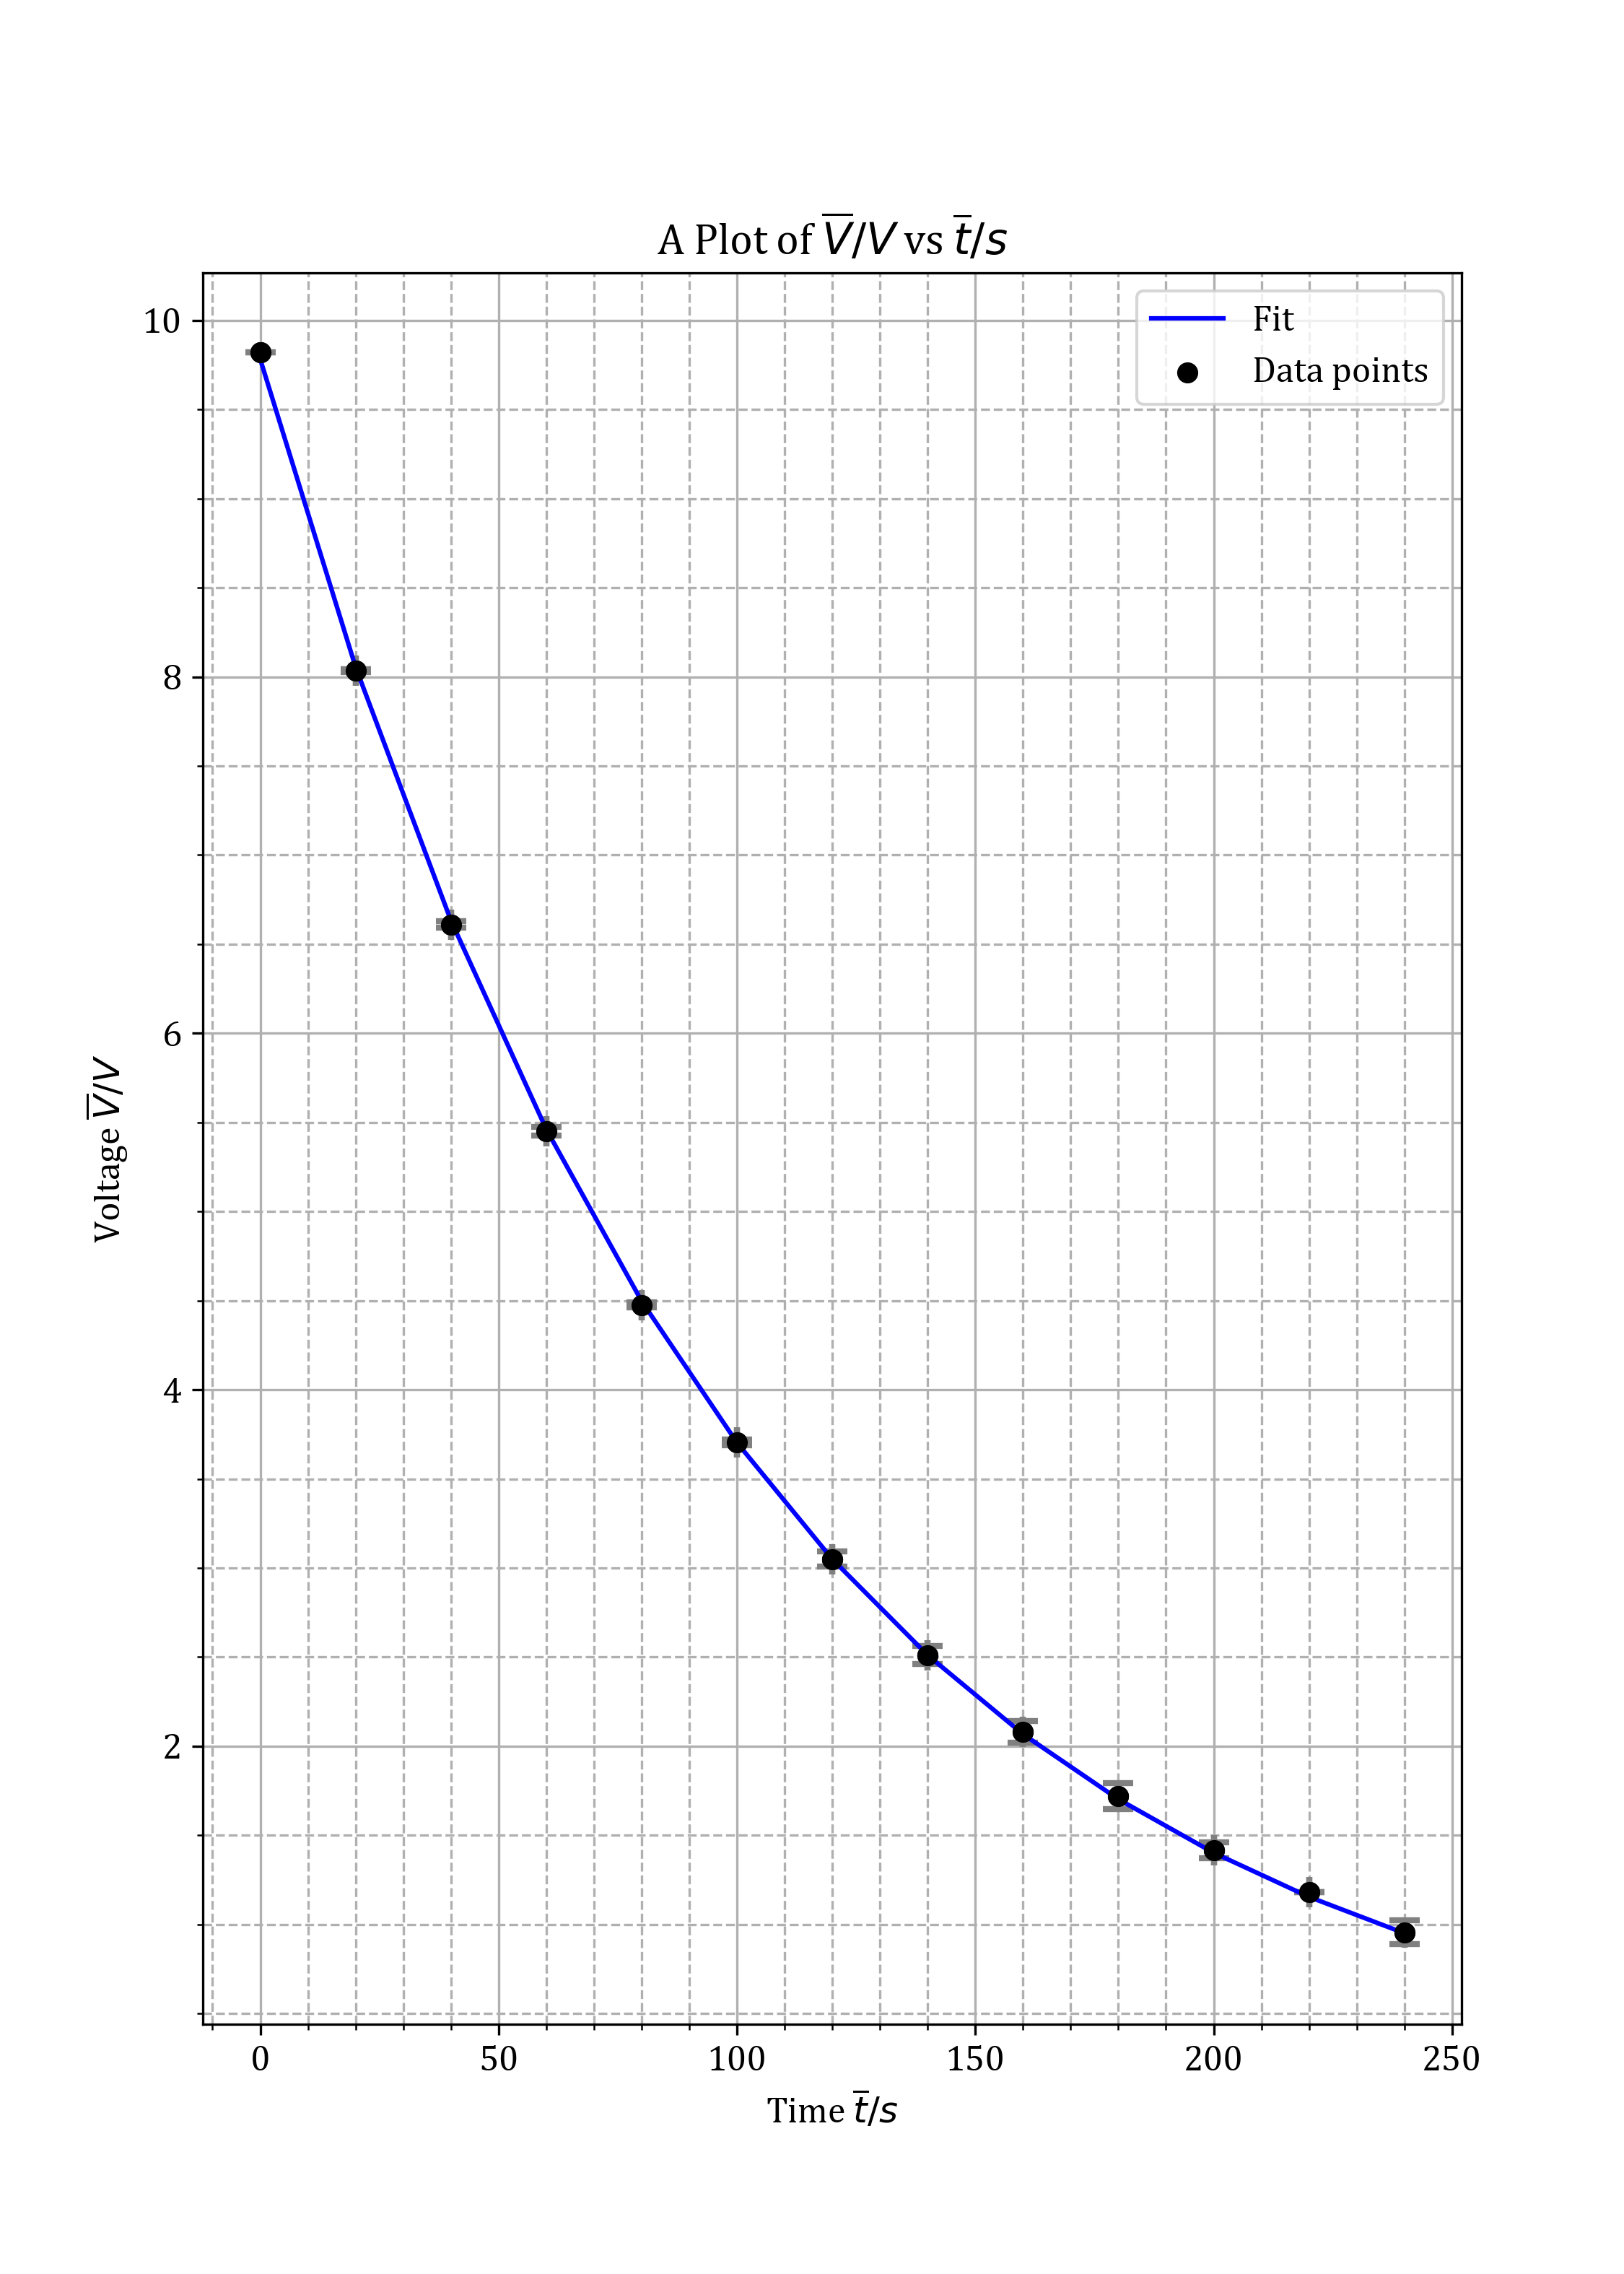
\includegraphics[width=\textwidth]{Experiment0ExpPlot.png}
    \caption{Voltage against Time Exponential}
    \label{fig:Exponential Graph}
\end{figure}
    
\begin{figure}
    \centering
    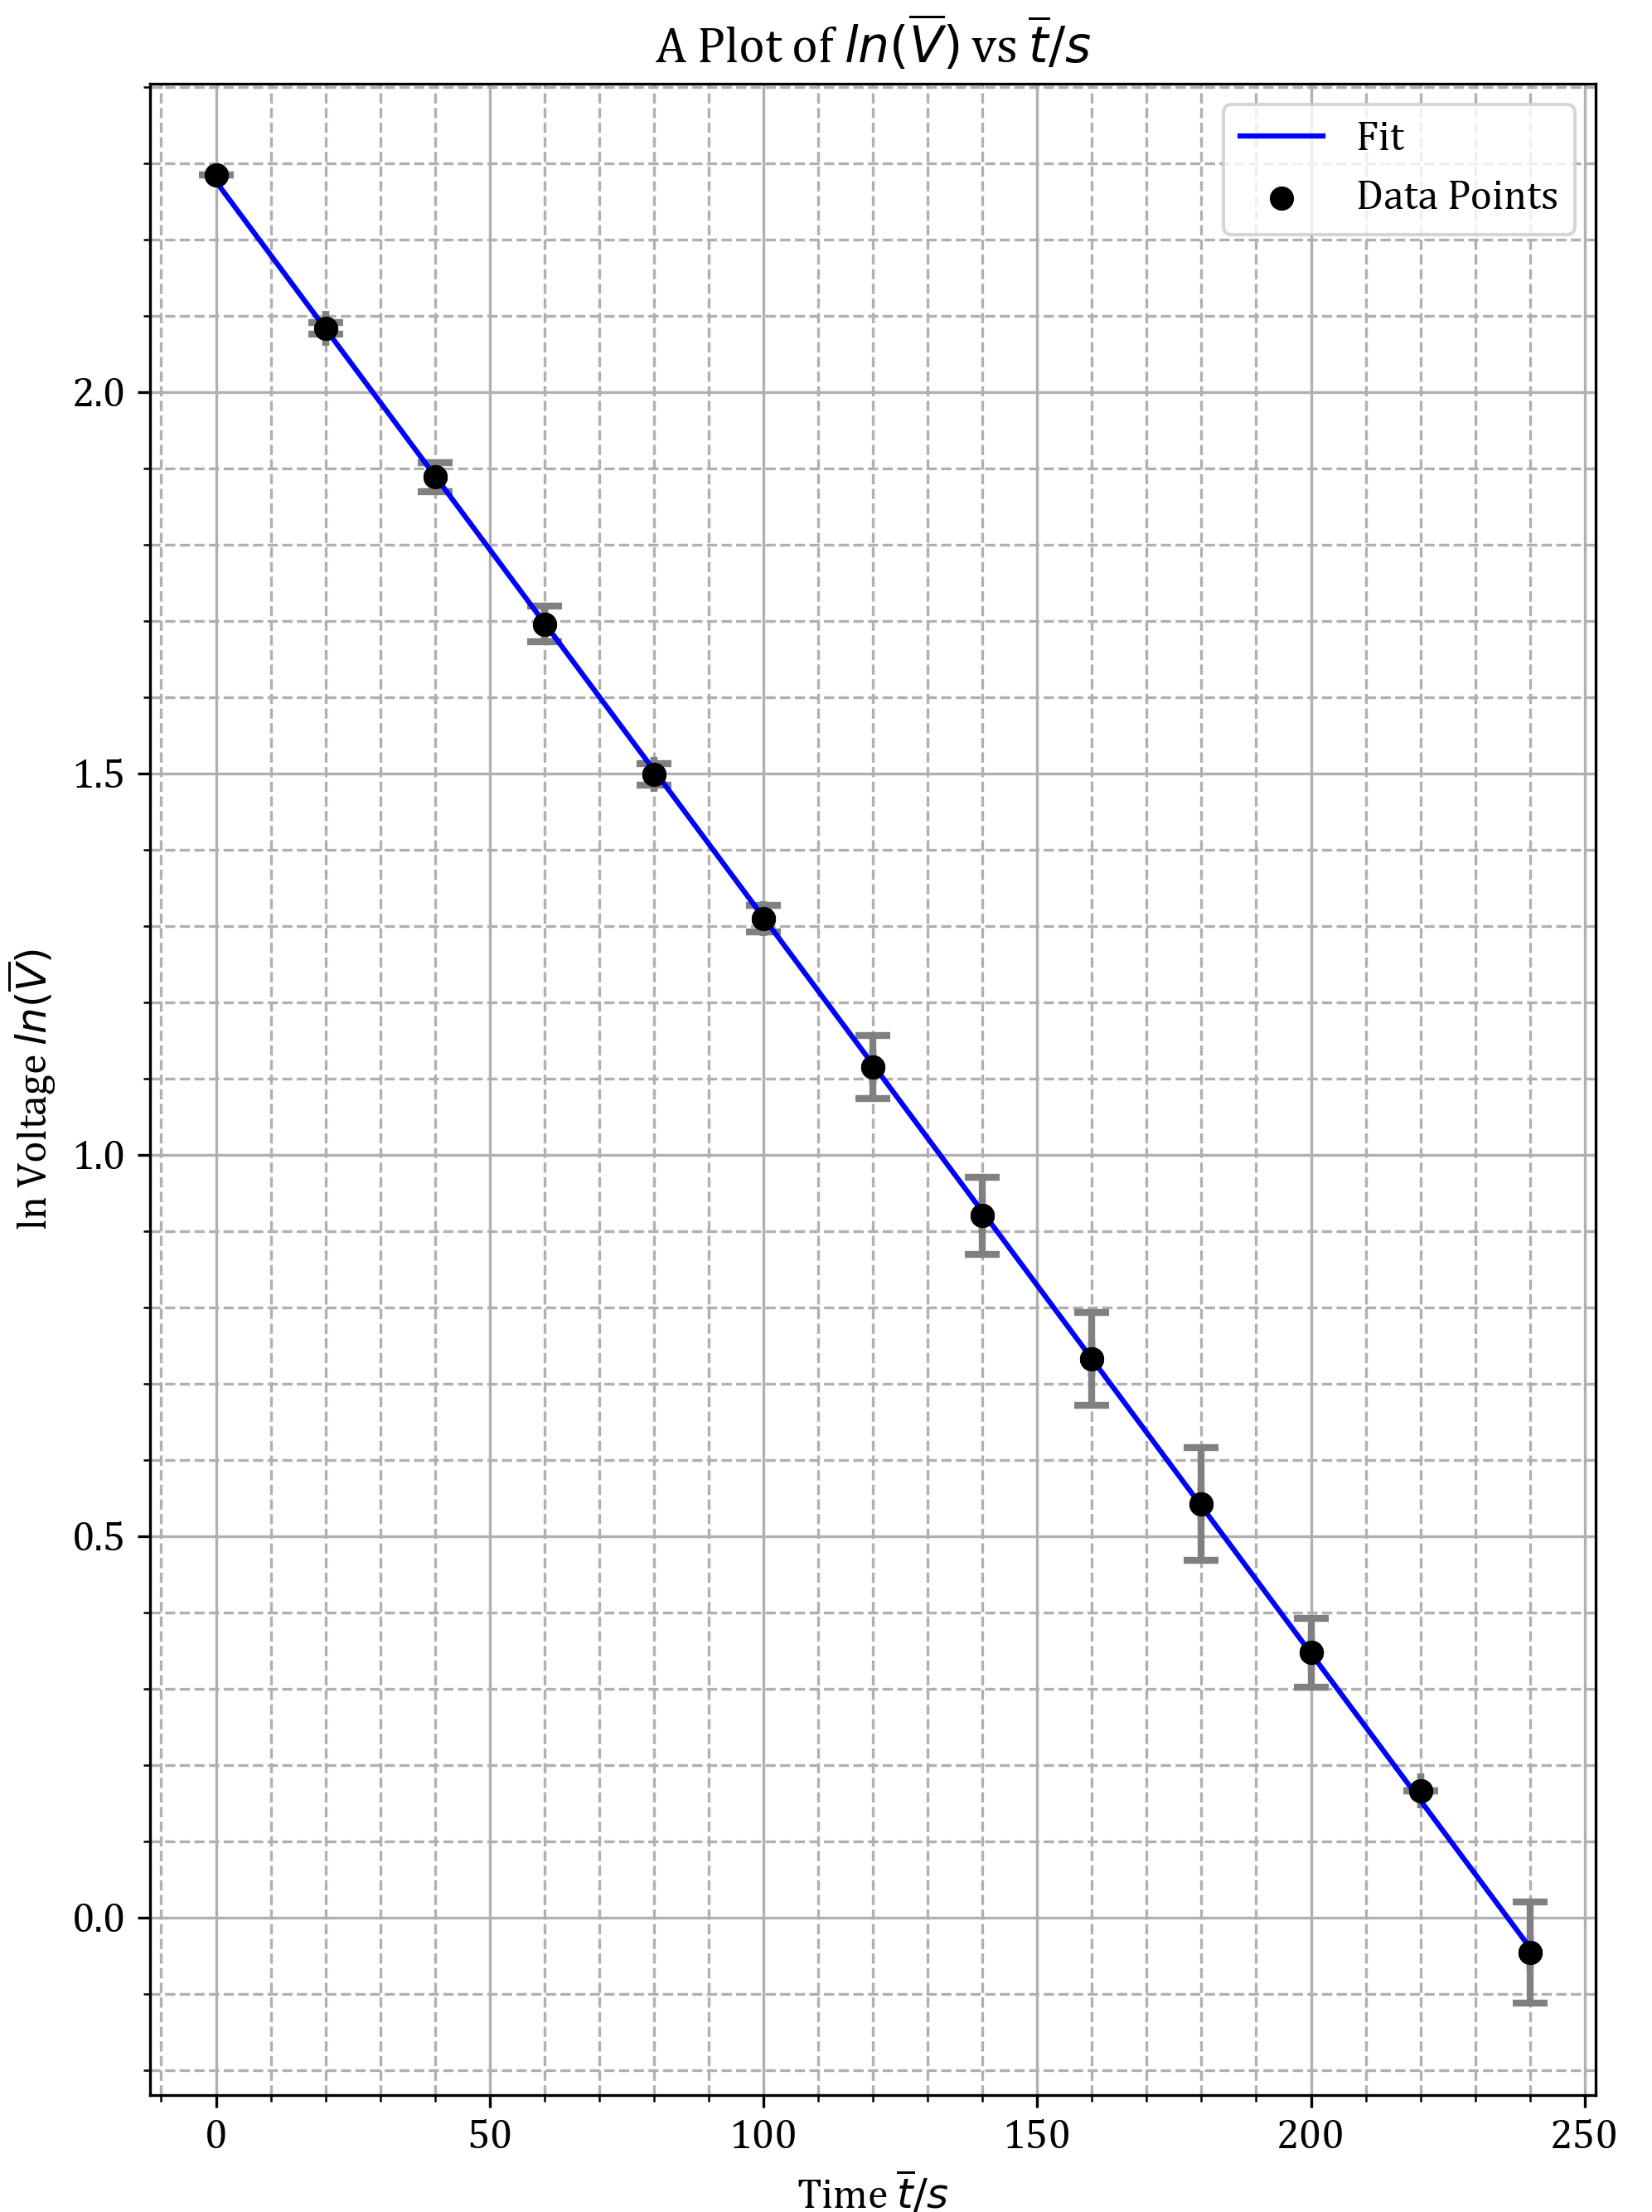
\includegraphics[width=\textwidth]{Experiment0LinearPlot.png}
    \caption{Voltage against Time Linear}
    \label{fig:Linear Graph}
\end{figure}

\section*{Data Analysis:}
The data collected was inputted into an excel sheet with corresponding headers for voltage and time, and the program was instructed to read the data from the excel sheet using the following code:
\begin{verbatim}
    data = pd.read_excel('Experiment 0.xlsx', 0)    
\end{verbatim}
In order to obtain the average of the data set for voltage and time the two following lines of code were used:

\begin{verbatim}
    average_v = 0.5 * (data['V1'] + data['V2']) 
    time = 0.5 * (data['t1'] + data['t2'])
\end{verbatim}    
These values were then used in the curve fit function from scipy.optimise in order to obtain the correct curve fit for the data points collected, using the following lines of code:
\begin{verbatim}
    def fit_ft(t, v0, t_c):
    return v0 * np.exp(-t/t_c)
 
    popt, pcov = curve_fit(fit_ft, time, average_v, p0=(2,2))
    fitted_line = fit_ft(time, popt[0], popt[1])
\end{verbatim}
Where the values obtained by the optimisation matrix are the values for $\text{V}_0$ and T and these were used to fit the line to the point, while the values from the co-variance matrix were used in order to obtain the error values of both $\text{V}_0$ and T. 
Furthermore, the change in voltage and time values was calculated by first finding the standard deviation of both voltage and time and then using the following equations:
\begin{equation}
    \Delta V = t_{\alpha, n-1} \frac{s}{\sqrt{n}}
\end{equation}
\begin{equation}
    \Delta T = t_{\alpha, n-1} \frac{s}{\sqrt{n}}
\end{equation}
In the case for the exponential fit these were obtained by calling the correct locations in the co-variance matrix from the curve fit function by the following code:
\begin{verbatim}
    print(f'V0 is : {popt[0]}, with an error of: {(pcov[0][0])**0.5}')
    print(f'T is : {popt[1]}, with an error of: {(pcov[1][1])**0.5}')
\end{verbatim}
The values obtained were as follows:\\
\indent$\text{V}_0 \text{ is: 9.7825V, with an error of: 0.0149V.}$\\
\indent$\text{T} \text{ is: 102.9451s, with an error of: 0.2609s.}$\\
The change in voltage and time were computed with the following lines of code:
\begin{verbatim}
    standard_deviation_V = np.std([data['V1'], data['V2']], axis=0, 
    ddof=1)
    delta_v = 12.7 * standard_deviation_V / np.sqrt(2)
    
    standard_deviation_t = np.std([data['t1'], data['t2']], axis=0, 
    ddof=1)
    delta_t = 12.7 * standard_deviation_t / np.sqrt(2)
    
    delta_v /= average_v
    delta_t /= time
\end{verbatim}
These lines of code provided the error bars in both the y-axis and x-axis respectively. 
For the linear graph of voltage against time the same procedure was followed to obtain the data and averages. However, in order to linearize the data, the natural log of the voltages was taken by using the following line of code:
\begin{verbatim}
    lnV = np.log(average_v) 
\end{verbatim}
The log of voltage, and time were plotted against each other and the data from the straight-line graph was then obtained by using the polyfit function. In this case the gradient would be equal to $-\frac{1}{\text{T}}$ and the y-intercept is $\text{lnV}_0$. The variables and the co-variance matrix were obtained and converted into $\text{V}_0$ and T by the following lines of code:
\begin{verbatim}
    coeffs, V = np.polyfit(time, lnV, 1, cov=True)
    vf = np.exp(coeffs[1]) 
    Tf = (np.power(coeffs[0], -1)) * -1
\end{verbatim}
The co-variance matrix obtained was then used to obtain the error margins of $\text{V}_0$ and T by finding the root of the values previously obtained:
\begin{verbatim}
    error_vf = np.sqrt(V[1][1]) 
    error_Tf = np.sqrt(V[0][0]) 
\end{verbatim}
This resulted in the values being as follows:\\
\indent$\text{V}_0 \text{ is: 9.7387V, with an error of: 0.0029V.}$\\
\indent$\text{T} \text{ is: 103.6399s, with an error of: 2.0680}{\times}10^{-5}\text{s.}$\\
The trend line was then plotted with the use of the poly1d function, and aforementioned the gradient and the y-intercept in order to get the line of best fit with this data. This was done using the following lines of code:
\begin{verbatim}
    poly_function = np.poly1d(coeffs)
    trendline = poly_function(time)
\end{verbatim}
The precision for all values obtained was calculated using the following formula:
\begin{equation}
    Precision = \frac{Total Error}{Experimental Value}{\times}100\%
\end{equation}
For $\text{V}_0$ from the exponential fit we get:
\begin{equation*}
    Precision = \frac{0.0149}{9.7826}{\times} 100\%
\end{equation*}
\begin{equation*}
    Precision = 0.1523\%
\end{equation*}
While for $\text{V}_0$ from the linear fit:
\begin{equation*}
    Precision = \frac{0.0029}{9.7387}{\times} 100\%
\end{equation*}
\begin{equation*}
    Precision = 0.0298\%
\end{equation*}
For T from the exponential fit we get:
\begin{equation*}
    Precision = \frac{0.2609}{102.9451}{\times} 100\%
\end{equation*}
\begin{equation*}
    Precision = 0.2534\%
\end{equation*}
While for T from the linear fit:
\begin{equation*}
    Precision = \frac{2.0680{\times}10^{-5}}{103.6399}{\times} 100\%
\end{equation*}
\begin{equation*}
    Precision = 1.9954{\times} 10^{-5}\%
\end{equation*}

\section*{Discussion:}
As the discharging of the capacitor yields two graphs, one of which is an exponential and another being linear, two methods to fit the data to the trend line were used. First, the data gathered was fitted to the exponential curve by the use of the curve fit function from the scipy.optimize library. In order for the curve fit function to work properly a function with a known value and the unknown values is first defined and from there it is recalled later in the curve fit with the comparison variable and a predefined initial condition so as to narrow down the search field. This can be clearly seen in these lines of code \parencite{Scipy.org_CurveFit}:
\begin{verbatim}
    def fit_ft(t, v0, t_c):
    return v0 * np.exp(-t/t_c)

    popt, pcov = curve_fit(fit_ft, time, average_v, p0=(2,2))
\end{verbatim}
The pcov variable returns the co-variance matrix of the function which then calls certain positions in the matrix are called in order to obtain the error values for $\text{V}_0$ and T for the exponential fit. These were found to be:\\
\indent$\text{V}_0 \text{ = 9.7826V \textpm 0.0149V} $\\
\indent$\text{T} \text{ = 102.9451s \textpm 0.2609s}$\\
Additionally, the data gathered was first linerized with the use of the natural log in order to remove the exponential in the general equation, which resulted in the following equation:
\begin{equation}
    \mbox{ln}V = -\frac{1}{\mbox{T}}t + \mbox{lnV}_0
    \end{equation}
Which gives rise to the gradient being $-\frac{1}{\mbox{T}}$ and the y-intercept being $\mbox{lnV}_0$, that were obtained from the function polyfit. The polyfit function will take two inputs and will return the polynomial function, and in this case as the polynomial in question is a straight line graph, it will return the coefficient m, which is the gradient, and c, which is the y-intercept. In addition as the cov, part of the function is set to true therefore will return a matrix with the co-variance values which then can be used in order to obtain the error values for the gradient and y-intercept \parencite{Numpy.Polyfit}. The coefficients obtained from this function were then plugged into another function called poly1d which will create the line of best fit for the coefficients provided, as can be seen in the following lines \parencite{Numpy.Poly1D}:
\begin{verbatim}
    poly_function = np.poly1d(coeffs)
    trendline = poly_function(time)
\end{verbatim}
In order to obtain the error values for both $\text{V}_0$ and T, the square root of the values in the corresponding locations in the co-variance matrix were taken as shown in these lines :
\begin{verbatim}
    error_vf = np.sqrt(V[1][1])
    error_Tf = np.sqrt(V[0][0])
\end{verbatim}
These resulted in the following values for $\text{V}_0$ and T:\\
\indent $\text{V}_0 \text{ = 9.7387V \textpm 0.0029V}$\\
\indent $\text{T} \text{ = 103.6399s \textpm 2.0680}{\times}10^{-5}\text{s}$
\smallbreak
\noindent The precision values for $\text{V}_0$ were found to be $0.1523\%$ and 0.0298\% for the exponential fit and the linear fit respectively. The precision values for T were found to be $0.2534\%$ and $1.9954{\times} 10^{-5}$ for the exponential fit and linear fit respectively. The slight difference between the two time constant values signifies that the data collected correlates between both fits obtained from the data gathered. The low values for precision for the time constants is also very significant as this means that the data gathered is quite precise.
\smallbreak
\noindent As can be seen in both Figure 1 on page \pageref{fig:Exponential Graph} and Figure 2 on page \pageref{fig:Linear Graph}, the error bars present, not only vary between each figure but also between each point in their respective figure. In Figure ~\ref{fig:Exponential Graph} on page \pageref{fig:Exponential Graph} the error bars present, are quite close to each other with respect to the x-axis and y-axis, which means that the data gathered does not fluctuate as much. However, one must consider the fact that the exponential axes have a much larger range and thus the actual size of the error bars is not that apparent. In Figure \ref{fig:Linear Graph} on page \pageref{fig:Linear Graph} the error bars of each point are more visible as the range of the axes is much lower then that in Figure \ref{fig:Exponential Graph} on page \pageref{fig:Exponential Graph}. As one can see the error bars in this figure vary from minimal to having a greater difference. The greater difference in the error bars, suggests a greater difference in variation of the data points and vice-versa. 

\printbibliography[title = {References:}]

\section*{Appendix:}
\begin{verbatim}
import matplotlib.pyplot as plt
from scipy.optimize import curve_fit
import pandas as pd
import numpy as np

# calling excel sheet for data
data = pd.read_excel('Experiment 0.xlsx', 0)    
# calling each column of voltage to find average voltage
average_v = 0.5 * (data['V1'] + data['V2'])     
# calling each column of time to find average time
time = 0.5 * (data['t1'] + data['t2'])          


# defining the function to return voltage and finding V0 and T 
def fit_ft(t, v0, t_c):                         
# returning the voltage value    
    return v0 * np.exp(-t/t_c)                  
 
# using curve-fit and the function in order to obtain a curve
popt, pcov = curve_fit(fit_ft, time, average_v, p0=(2, 2))  
# using called time in order to obtain optimised values for unknowns
fitted_line = fit_ft(time, popt[0], popt[1])                
 
# obtaining the value of opt value of V0 and its error value
print(f'V0 is : {popt[0]}, with an error of: {(pcov[0][0])**0.5}')     
# obtaining the value of opt value of T and its error value
print(f'T is : {popt[1]}, with an error of: {(pcov[1][1])**0.5}')      

# obtaining std of V0 
standard_deviation_V = np.std([data['V1'], data['V2']], axis=0, ddof=1)  
# obtaining the change in value of V0 wrt pop
delta_v = 12.7 * standard_deviation_V / np.sqrt(2)                       
 
# obtaining std of T
standard_deviation_t = np.std([data['t1'], data['t2']], axis=0, ddof=1)  

# obtaining the change in value of T wrt pop
delta_t = 12.7 * standard_deviation_t / np.sqrt(2)                       
 
# obtaining the change in value of V0 wrt average
delta_v /= average_v                                                     
# obtaining the change in value of T wrt average
delta_t /= time                                                          
 
# defining the font to be used
plt.rcParams["font.family"] = "Cambria"                                  
# defining the size of the font
plt.rcParams["font.size"] = 12                                           
# defining the font to be normal
plt.rcParams["font.weight"] = "normal"                                   
 
# defining the size of the figure
f = plt.figure(figsize=(7.5, 10.5))                                      
# defining he error bars for each point
plt.errorbar(time, average_v, xerr=delta_t, yerr=delta_v, fmt='o', color='k', 
elinewidth=2, capthick=2, capsize=5, ecolor='grey')                                              
# defining the scatter plot
plt.scatter(time, average_v, color='k', label='Data points')             
# plotting the curve
plt.plot(time, fitted_line, 'b-', label='Fit')                           
 
# showing minor lines on the graph
plt.minorticks_on()
# defining the style of the major lines
plt.grid(b=True, which='major', linestyle='-')
# defining the style of the minor lines
plt.grid(b=True, which='minor', linestyle='--')

# showing the legend
plt.legend()                                                             
# defining the x-axis label
plt.xlabel(r"Time $t/s$")                                                
# defining the y-axis label
plt.ylabel(r"Voltage $V/V$")                                             
# defining the title of the graph
plt.title('A Plot of V/V vs t/s')
# saving the figure
plt.savefig('Experiment0ExpoGraph.png', dpi=300)
 
plt.show()

# Linear Graph 
# calling the excel file for the data 
data = pd.read_excel('Experiment 0.xlsx', 0)
# finding the average of each column of voltage
average_v = 0.5 * (data['V1'] + data['V2'])
# finding the average of each column of time
time = 0.5 * (data['t1'] + data['t2'])

# finding the log of the average voltage 
lnV = np.log(average_v)

# using polyfit in order to obtain m and c and covariance 
coeffs, V = np.polyfit(time, lnV, 1, cov=True)
# using c to find V0
vf = np.exp(coeffs[1])
# using m to find T
Tf = (np.power(coeffs[0], -1)) * -1 


# calling the position in the covariance matrix as the error value of V0 
error_vf = np.sqrt(V[1][1]) 
# calling the position in the covariance matrix as the error value of T
error_Tf = np.sqrt(V[0][0])

# displaying V0 with error 
print(f'lnV is: {vf}, with an error of: {error_vf}')
# displaying T with error
print(f'T is: {Tf}, with an error of: {error_Tf}')

# finding the std of V 
standard_deviation_V = np.std([data['V1'], data['V2']], axis=0, ddof=1)
# finding the change in V wrt pop
delta_v = 12.7 * standard_deviation_V / np.sqrt(2)

# finding the std of t 
standard_deviation_t = np.std([data['t1'], data['t2']], axis=0, ddof=1)
# finding the change in t wrt pop
delta_t = 12.7 * standard_deviation_t / np.sqrt(2)

# updating the change in V
delta_v /= average_v
# updating the change in t
delta_t /= time

# using the gradient and y-intercept to calculate the best straight line 
poly_function = np.poly1d(coeffs)
trendline = poly_function(time)

# defining the font to be used 
plt.rcParams["font.family"] = "Cambria"

# defining the font size
plt.rcParams["font.size"] = 12 
# defining the thickness of the font
plt.rcParams["font.weight"] = "normal"

# defining the size of the figure
f = plt.figure(figsize=(7.5, 10.5))
# plotting the error bars of each point
plt.errorbar(time, lnV, xerr=delta_t, yerr=delta_v, fmt='o', color='k', 
elinewidth=2, capthick=2,capsize=5, ecolor='grey')
# plotting the scatter graph
plt.scatter(time, lnV, color='k', label='Data Points')  
# plotting the line
plt.plot(time, trendline, color='b', label='Fit')

# turning on the minor lines 
plt.minorticks_on() 

# defining the style for major line
plt.grid(b=True, which='major', linestyle='-')     
# defining the style for minor lines
plt.grid(b=True, which='minor', linestyle='--')    
# displaying the legend
plt.legend()                                       
# defining the x-axis label
plt.xlabel(r"Time $\overline{t}/s$")                          
# defining the y-axis label
plt.ylabel(r"ln Voltage $ln(\overline{V})$")                  
# defining the graph title
plt.title(r'A Plot of $ln(\overline{V})$ vs $\overline{t}/s$') 
# saving the figure
plt.savefig('Experiment0LinearPlot.png', dpi=300)      

# showing the plotted graph 
plt.show()                                         

\end{verbatim}[\fontsize{12pt}{12pt}]

\end{document}
